
\serie{Relations trigonométriques}

\begin{exercice}
En utilisant la calculatrice, donner la valeur arrondie à 1° près de l'angle aigu $\alpha$.

\begin{multicols}{2}
\begin{enumerate}
\item $\sin(\alpha)=0,35$

\item $\tan(\alpha)=2,7$

\item $\cos(\alpha)=0,9$

\item $\sin(\alpha)=\dfrac{2}{3}$

\end{enumerate}
 \end{multicols}
\end{exercice}

\begin{exercice}
On considère des angles aigus $a$ et $b$
\begin{enumerate}
\item Supposons que $\sin(a)=0,6$. A l'aide d'une calculatrice, calculer $\cos(a)$ et $\tan(a)$.
\item Supposons que $\tan(b)=\sqrt{3}$. En déduire $b$ à l'aide d'une calculatrice.
\end{enumerate}
\end{exercice}

\begin{exercice}
On dit qu'une route monte à $15\%$ si on monte de 15 m lorsqu'on avance de 100 m sur la route.

A quel rapport  trigonométrique correspond $\dfrac{15}{100}$ pour l'angle formé par la route et l'horizontale?
\end{exercice}

\begin{exercice}
$ABC$ est un triangle rectangle en $B$.

On donne : $BC=7,8$cm et $AC=10,4$cm.
\begin{enumerate}
\item Calculer $\sin\left(\widehat{BAC} \right)$.
\item En déduire la mesure de l'angle $\widehat{BAC}$ à 1° près. 
\end{enumerate}
\end{exercice}

\begin{exercice}
$IJK$ est un triangle rectangle en $J$.\\
On donne : $IJ=66,4$cm et $JK=24,9$cm.
\begin{enumerate}
\item Calculer $\tan\left(\widehat{JIK} \right)$.
\item En déduire la mesure de l'angle $\widehat{JIK}$ à 1° près. 
\end{enumerate}
\end{exercice}

\begin{exercice}
$ABC$ est un triangle rectangle en $B$.\\
On a : $AC=12$cm et $\sin(\widehat{BAC})=0,8$.
Calculer $BC$.
\end{exercice}

\begin{exercice}
$KLM$ est un triangle rectangle en $L$.\\
On a : $LM=4,2$cm et $\tan(\widehat{LKM})=1,5$.
Calculer $KL$.
\end{exercice}

\begin{exercice}
Soit $EFG$ un triangle rectangle en $E$ tel que $EF=7$ et $EG=9$.\\
Calculer la mesure de chacun des angles aigus du triangle $EFG$. Donner vos résultat arrondis au degré.
\end{exercice}

\begin{exercice}
Soit $ABC$ un triangle rectangle en $A$. L'angle $\widehat{ABC}$ mesure $55\textrm{\degre}$ et la longueur du côté $[AC]$ mesure $17cm$.\\
Calculer les longueurs $BC$ et $AB$. Donner les valeurs arrondis au dixième.
\end{exercice}

\begin{exercice}
Une échelle de $3,50m$ arrive à $3,30m$ de hauteur sur un mur vertical. 
Quelle angle fait l'échelle avec le sol? Donner votre résultat arrondi au dixième près.
\end{exercice}

\begin{exercice}
Un observateur, qui a les yeux à 1,63m du sol vise le sommet d'un immeuble situé à 31m de lui. On a la situation suivante
\begin{center}
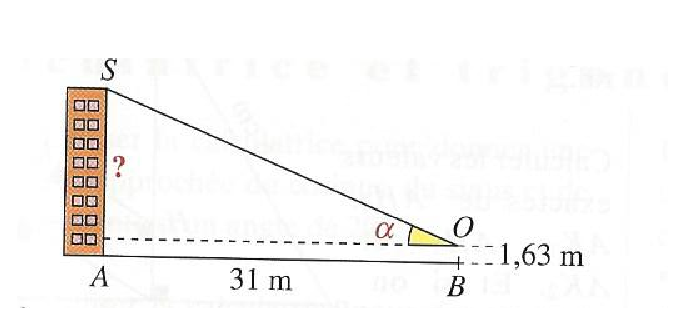
\includegraphics[scale=0.7]{Trigonometrie/figures/observateur.eps}
\end{center}
On mesure un angle $\alpha$ de $37\textrm{\degre}$.

Déterminer une valeur arrondie au dixième de la hauteur de l'immeuble.
\end{exercice}

\begin{exercice}
Jacques navigue le long d'une falaise. Pour des questions de sécurité, il ne doit pas aller au delà du point $C$. I a jeté l'ancre au point $B$. On a $SH=100m$, $\widehat{HCS}=75\textrm{\degre}$, $\widehat{HBS}=65\textrm{\degre}$. À quelle distance du point C le bateau de Jacques se trouve t-il? Donner la valeur approchée par excès au millième de mètre près.
\begin{center}
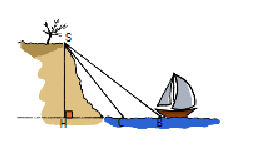
\includegraphics[scale=1]{Trigonometrie/figures/bateau_trigo.eps}
\end{center}
\end{exercice}

\begin{exercice}
Sur la figure $BD=5$cm.

Calculer la longueur de chacun des côtés du quadrilatère $ABCD$ à 1 mm près.

\begin{center}
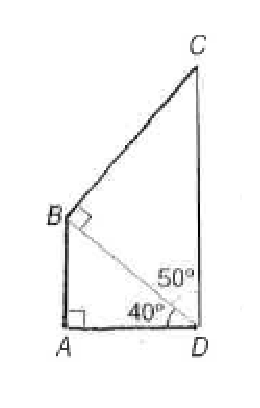
\includegraphics[scale=0.6]{Trigonometrie/figures/quadrilatere.eps}
\end{center}
\end{exercice}

\serie{Propriétés}

\begin{exercice}
\textbf{Vrai ou faux?}

Voici ce qu'a écrit Raoul sur sa copie:

\begin{center}
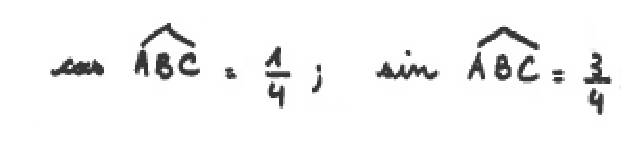
\includegraphics[scale=0.6]{Trigonometrie/figures/raoul.eps}
\end{center}
Cela peut-il être exact? Justifier votre réponse.
\end{exercice}

\begin{exercice}
Calculer la valeur exacte de $\tan(\alpha)$ dans chacun des cas:

\begin{multicols}{2}
\begin{enumerate}
\item $\sin(\alpha)=2\cos(\alpha)$
\item $\cos(\alpha)=4\sin(\alpha)$
\item $\cos(\alpha)=\dfrac{\sin(\alpha)}{5}$
\item $\cos(\alpha)=\dfrac{2}{3}\sin(\alpha)$
\end{enumerate}
\end{multicols}
\end{exercice}

\begin{exercice}
Soit $\alpha$ un angle aigu tel que $\sin(\alpha)=\frac{1}{4}$
\begin{enumerate}
	\item Déterminer $\cos(\alpha)$ (on admet que $\cos(\alpha)>0$)
	\item Déterminer $\tan(\alpha)$
\end{enumerate}
\end{exercice}

\begin{exercice}
Calculer la valeur exacte de $\cos(\alpha)$ et de $\tan(\alpha)$ sachant que $\alpha$ est un angle aigu tel que $\sin(\alpha)=\dfrac{\sqrt{6}-\sqrt{2}}{4}$.
\end{exercice}

\begin{exercice}
Soit $x$ un angle aigu. Démontrer que 

$(\cos(x)+\sin(x))^2=1+2\sin(x)\cos(x)$
\end{exercice}

\begin{exercice}
Montrer que $1+\tan^2(x)=\dfrac{1}{\cos^2(x)}$ pour tout $x$ tel que $\cos(x)\ne 0$.
\end{exercice}

\begin{exercice}
\begin{enumerate}
	\item Soit $x$ un angle aigu tel que $\cos(x)=\dfrac{2}{3}$.
	
	 Déterminer la valeur exacte de $\sin(x)$ (on admet que $\sin(x)>0$).
	\item Montrer que $\tan(x)\cdot\sin(x)+\cos(x)=\dfrac{1}{\cos(x)}$ pour tout $x$ tel que $\cos(x)\ne 0$
\end{enumerate}
\end{exercice}

\begin{exercice}
A l'aide d'un triangle rectangle:
\begin{enumerate}
	\item Démontrer que $\cos(20\textrm{\degre})=\sin(70\textrm{\degre})$ et que $\sin(20\textrm{\degre})=\cos(70\textrm{\degre})$.
	\item De façon générale, démontrer que, si $\alpha$ et $\beta$ sont complémentaires, alors $\cos(\alpha)=\sin(\beta)$ et $\sin(\alpha)=\cos(\beta)$.
\end{enumerate}
\end{exercice}

\begin{exercice}
\begin{enumerate}
	\item Calculer la hauteur d'un triangle équilatéral de côté 1;
		\item En déduire les valeurs exactes de $\sin(60\textrm{\degre})$ et de $\cos(60\textrm{\degre})$;
	\item Puis en déduire les valeurs exactes de $\sin(30\textrm{\degre})$ et de $\cos(30\textrm{\degre})$.

\end{enumerate}
\end{exercice}

\begin{exercice}
Sur la figure, démontrer que : $TU \times TR=TS^2$.
\begin{center}
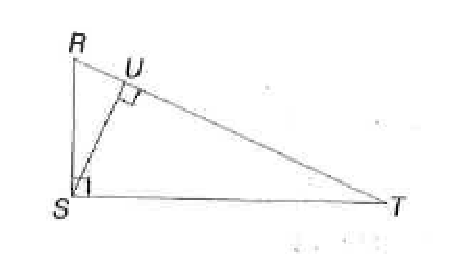
\includegraphics[scale=0.6]{Trigonometrie/figures/triangle.eps}
\end{center}
\end{exercice}

\serie{Divers}

\begin{exercice}

On considère un triangle $ABC$ rectangle en $B$ et un triangle $BCD$ rectangle en $D$ comme sur la figure tels que $BD=4$ cm, $BA=6$ cm et $\widehat{DBC}=60\textrm{\degre}$ (la figure n'est pas représentée en vraie grandeur)
\begin{enumerate}
\item Montrer que $BC=8cm$
\item Calculer $CD$.
\item Calculer $AC$
\item Déterminer la valeur arrondie au degré de $\widehat{BAC}$.
\end{enumerate}
\begin{center}
\definecolor{zzttqq}{rgb}{0.6,0.2,0.}
\definecolor{qqqqff}{rgb}{0.,0.,1.}
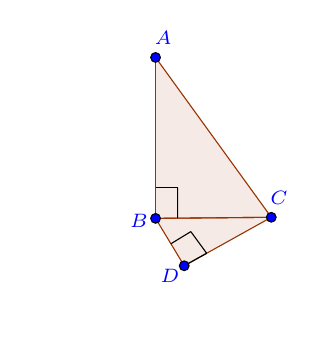
\begin{tikzpicture}[scale=0.7][line cap=round,line join=round,>=triangle 45,x=1.0cm,y=1.0cm]
\clip(-1.,-1.) rectangle (4,4.5);
\fill[color=zzttqq,fill=zzttqq,fill opacity=0.1] (1.32,3.96) -- (1.32,1.04) -- (3.42,1.06) -- cycle;
\fill[color=zzttqq,fill=zzttqq,fill opacity=0.1] (1.32,1.04) -- (1.84,0.18) -- (3.42,1.06) -- cycle;
\draw [color=zzttqq] (1.32,3.96)-- (1.32,1.04);
\draw [color=zzttqq] (1.32,1.04)-- (3.42,1.06);
\draw [color=zzttqq] (3.42,1.06)-- (1.32,3.96);
\draw [color=zzttqq] (1.32,1.04)-- (1.84,0.18);
\draw [color=zzttqq] (1.84,0.18)-- (3.42,1.06);
\draw [color=zzttqq] (3.42,1.06)-- (1.32,1.04);
\draw (1.32,1.6)-- (1.72,1.6);
\draw (1.5986376237623765,0.579176237623762)-- (1.96,0.8);
\draw (1.96,0.8)-- (2.2473180873180874,0.40686070686070686);
\draw (1.32,1.6)-- (1.72,1.6);
\draw (1.72,1.6)-- (1.719963722111373,1.0438091783058225);
\draw (2.2473180873180874,0.40686070686070686)-- (1.84,0.18);
\begin{scriptsize}
\draw [fill=qqqqff] (1.32,3.96) circle (2.5pt);
\draw[color=qqqqff] (1.46,4.32) node {$A$};
\draw [fill=qqqqff] (1.32,1.04) circle (2.5pt);
\draw[color=qqqqff] (1.02,1.) node {$B$};
\draw [fill=qqqqff] (3.42,1.06) circle (2.5pt);
\draw[color=qqqqff] (3.56,1.42) node {$C$};
\draw [fill=qqqqff] (1.84,0.18) circle (2.5pt);
\draw[color=qqqqff] (1.58,0.) node {$D$};
\end{scriptsize}
\end{tikzpicture}
\end{center}
\end{exercice}

\begin{exercice}
$EDF$ est un triangle isocèle de sommet $E$ tel que $DF=6 cm$ et $ED=5 cm$.\\
Le symétrique de $D$ par rapport à $E$ est noté $G$.
\begin{enumerate}
\item Quelle est la nature du triangle $GDF$? Justifier.
\item Calculer l'angle $\widehat{EDF}$ à 1° près.
\end{enumerate}
\end{exercice}

\begin{exercice}
$RST$ est un triangle isocèle tel que : $RS=RT=7 cm$ et $\widehat{SRT}=37\textrm{\degre}$.\\
Calculer $ST$ à 1 mm près.
\end{exercice}

\begin{exercice}
ABC est un triangle rectangle. 

On note H le pied de la hauteur issue de A.

On $\widehat{ACB}=30\textrm{\degre}$ et AC=6 cm.

Calculer les valeurs \textbf{exactes} de BC, CH, AH, BA et BH.

\textbf{Ne pas utiliser le théorème de Pythagore.}
\end{exercice}

\begin{exercice}
Soit $ABC$ un triangle isocèle en $A$ tel que $BC=23,6$ cm et $\widehat{BAC}=42,5\textrm{\degre}$.\\
Déterminer l'aire du triangle $ABC$.\\
Indication : Considérer la hauteur issue de $A$ pour former deux triangles rectangles.
\end{exercice}

\begin{exercice}
Soit $ABC$ un triangle quelconque n'ayant que des angles aigus. On note $a=BC$, $b=AC$ et $c=AB$.
\begin{enumerate}
\item
\begin{itemize}
\item Démontrer que la hauteur issue de $A$ du triangle $ABC$ a pour longueur $b\cdot \sin(\widehat{ACB})$.
\item En déduire que l'aire $\mathcal{A}_{abc}$ du triangle $ABC$ est égale à $\dfrac{a\cdot b\cdot \sin(\widehat{ACB})}{2}$.
On peut montrer de la même manière que l'aire du triangle $ABC$ est égale à $\dfrac{b\cdot c\cdot \sin(\widehat{BAC})}{2}$ et à $\dfrac{a\cdot c\cdot \sin(\widehat{ABC})}{2}$
\end{itemize}
\item En déduire que 
\begin{align*}
\frac{\sin(\widehat{BAC})}{a}=\frac{\sin(\widehat{ABC})}{b}=\frac{\sin(\widehat{ACB})}{c}=\frac{2\cdot \mathcal{A}_{abc}}{a\cdot b\cdot c}
\end{align*}
\item On considère un triangle $ABC$ tel que $BC=7$ cm, $AB=5$ cm et $\widehat{BAC}=64\textrm{\degre}$.

Calculer les mesures des angles $ABC$ et $ACB$ arrondis au degré et la longueur $AC$ arrondie au dixième. 
\end{enumerate}
\end{exercice}

\begin{exercice}
Pour mesurer la hauteur de l'obélisque de la place de la Concorde à Paris, on a fait les relevés suivants : 
\begin{multicols}{3}
$\alpha=58.5\textrm{\degre}$
$\beta=35,1\textrm{\degre}$
$AB=18,7m$
\end{multicols}
Calculer la hauteur du monument.
\begin{center}
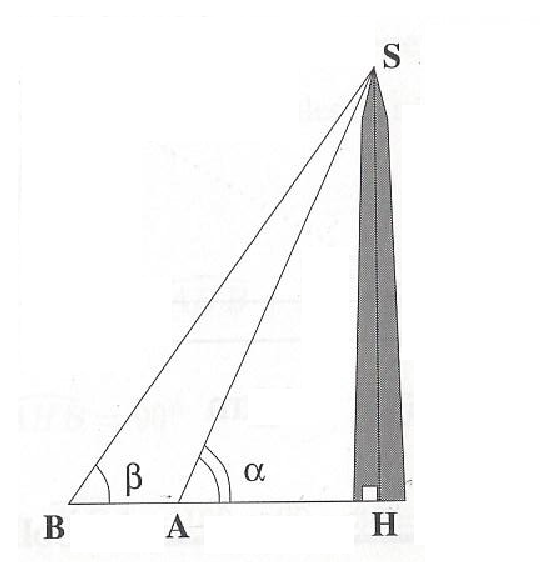
\includegraphics[scale=0.6]{Trigonometrie/figures/obelisque.eps}
\end{center}
\end{exercice}

\begin{exercice}
Pour mesurer la hauteur de la muraille d'un château, on prend les mesures suivantes : 
\begin{center}
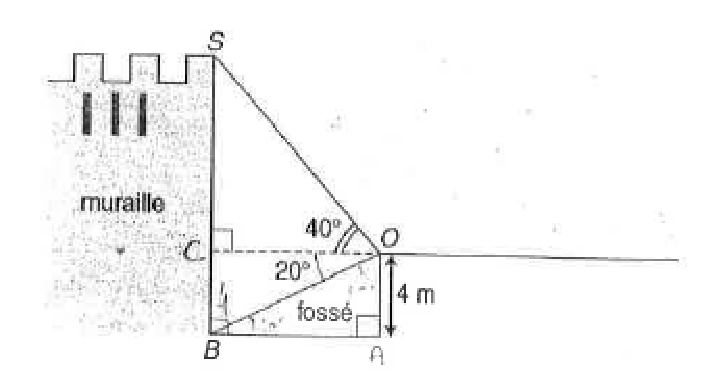
\includegraphics[scale=0.7]{Trigonometrie/figures/chateau.eps}
\end{center}
Calculer la hauteur $BS$.
\end{exercice}

\begin{exercice}
\begin{enumerate}
\item Construire en vraie grandeur un triangle $ABC$ tel que : $BC=6 cm$, $\widehat{ABC}=65\textrm{\degre}$ et $\widehat{ACB}=52\textrm{\degre}$.
\item 
\begin{enumerate}
\item Tracer la hauteur $[BH]$. Calculer $BH$ à 1 mm près.
\item Calculer la mesure de $\widehat{HBA}$. En déduire $AB$.
\end{enumerate}
\item Tracer la hauteur $[CK]$. Calculer $CK$ et $AC$ à 1 mm près.
\item Calculer l'aire et le périmètre du triangle $ABC$.
\end{enumerate}
\end{exercice}